% QUESTAO
Após determinar o outro cateto do triângulo retângulo abaixo, a sua área, em metros quadrados, fica:

\parbox{0.4\linewidth}{

% ALTERNATIVAS
$60$\,m$^2$
$120$\,m$^2$
$81$\,m$^2$
$64$\,m$^2$
$48$\,m$^2$

}\parbox{0.59\linewidth}{
\begin{center}
\vspace{-6mm}
\begin{tikzpicture}[ >=latex, scale=0.8 ]

\def\legA{}
\def\legB{}
\def\legC{}
\triangulo
{}	              {15}	               {0}
{$8$}		  {8}	               {0}
{$17$}	              {17}	               {0}

\end{tikzpicture}
\vspace{-9mm}
\end{center}
}


